\section{Setting up your M2T workspace}

Nowadays, \emph{no one} really writes a complex parser completely by hand.
Although this is sometimes still necessary\footnote{Some languages are syntactically quite challenging.} most parsers can be whipped up pretty quickly using context-free \emph{string grammars}\footnote{For simple cases, \emph{regular expressions} can also be used.} typically in EBNF\footnote{Extended Backus-Naur Form}.
ANTLR~\cite{ANTLR} is a tool that can generate a parser from a compact EBNF specification for a host of target programming languages, including Java.
Although ANTLR might not be the most efficient or powerful parser generator out there, it is open-source, well documented and supported, and allows for a pragmatic and quite elegant \emph{fallback} to Java when things get nasty and we have to resort to some dirty tricks.

The first step is preparing an Eclipse workspace according to our suggested workflow.

\begin{enumerate}
\item[$\blacktriangleright$] In Eclipse (preferably with an empty workspace), switch to our Moflon perspective and invoke the \texttt{New Metamodel} wizard (Fig.~\ref{fig:moca-1-NewMetamodelWizard}). 

%\usepackage{graphics} is needed for \includegraphics
\begin{figure}[!htbp]
\begin{center}
 
\includegraphics[width=0.3\textwidth]{pics/moca/1DictionaryMetaModel/1-NewMetamodelWizard.png}
  \caption{Invoking the \texttt{New Metamodel} wizard.}
  \label{fig:moca-1-NewMetamodelWizard}
\end{center}
\end{figure}

\item[$\blacktriangleright$] Choose ``Dictionary'' as project name and select \texttt{Add eMoflon languages} as depicted in Fig.~\ref{fig:moca-2-AddMocaSupport-ProjectName}. 

%\usepackage{graphics} is needed for \includegraphics
\begin{figure}[!htbp]
\begin{center}
 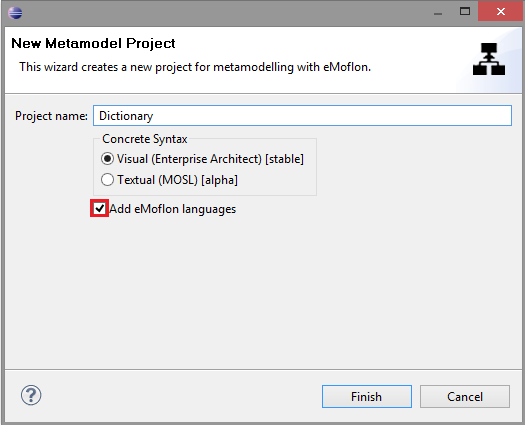
\includegraphics[width=0.7\textwidth]{pics/moca/1DictionaryMetaModel/2-AddMocaSupport-ProjectName.png}
  \caption{Add Metamodel project with MOCA support}
  \label{fig:moca-2-AddMocaSupport-ProjectName}
\end{center}
\end{figure}

\item[$\blacktriangleright$] After the project is created as usual (Fig. \ref{fig:moca-3-NewWizardResult}) double-click the EAP file to open it. 

%\usepackage{graphics} is needed for \includegraphics
\begin{figure}[!htbp]
\begin{center}
 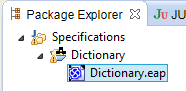
\includegraphics[width=0.3\textwidth]{pics/moca/1DictionaryMetaModel/3-WizardResult.png}
  \caption{Eclipse workspace after creating the \texttt{Dictionary} project}
  \label{fig:moca-3-NewWizardResult}
\end{center}
\end{figure}

\item[$\blacktriangleright$] In EA, the project is already populated with the metamodel for our generic tree.
To differentiate this from other trees (ANTLR parse tree and abstract syntax tree, XML DOM tree, \ldots) we shall refer to it as \texttt{MocaTree} (Fig.~\ref{fig:moca-4-eapContainsMocatreeWithExportFalse}).
Note that the \texttt{MocaTree} package has a special tagged value \texttt{Moflon::Export} that is set to \texttt{false}\footnote{Tagged values can be viewed in the \texttt{Tagged Values} view in EA (Fig.~\ref{fig:moca-4-eapContainsMocatreeWithExportFalse}).}.
This ensures that the package is \emph{ignored} when exporting.
As with all standard metamodels (e.g., Ecore or the SDM metamodel) the \texttt{MocaTree} package in EA should be regarded as read-only and is only required in the EA project so that SDMs can refer to the classes defined in the package.
The corresponding Java code is provided by our Eclipse plugin and is added automatically to the Java build path whenever necessary.

%\usepackage{graphics} is needed for \includegraphics
\begin{figure}[!htbp]
\begin{center}
 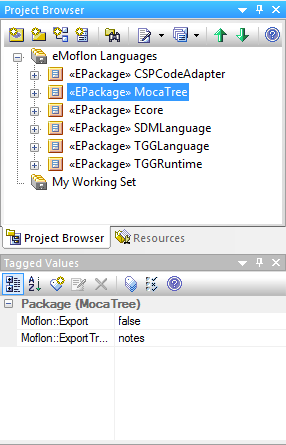
\includegraphics[width=0.4\textwidth]{pics/moca/1DictionaryMetaModel/4-eapContainsMocatreeWithExportFalse.png}
  \caption{\texttt{MocaTree} in default EA project}
  \label{fig:moca-4-eapContainsMocatreeWithExportFalse}
\end{center}
\end{figure}
\end{enumerate}

Go ahead and inspect the \texttt{MocaTree} metamodel (Fig.~\ref{fig:moca-tree}).
It basically combines concepts from a filesystem (folders and files), XML concepts (text-only nodes and attributes), and a general indexed\footnote{The index attribute in \texttt{TreeElement} can be used to demand a certain \emph{order} of nodes in an SDM, which is otherwise not guaranteed by default (order is in general non-deterministic).} containment hierarchy.

\begin{figure}[!htbp]
\begin{center}
 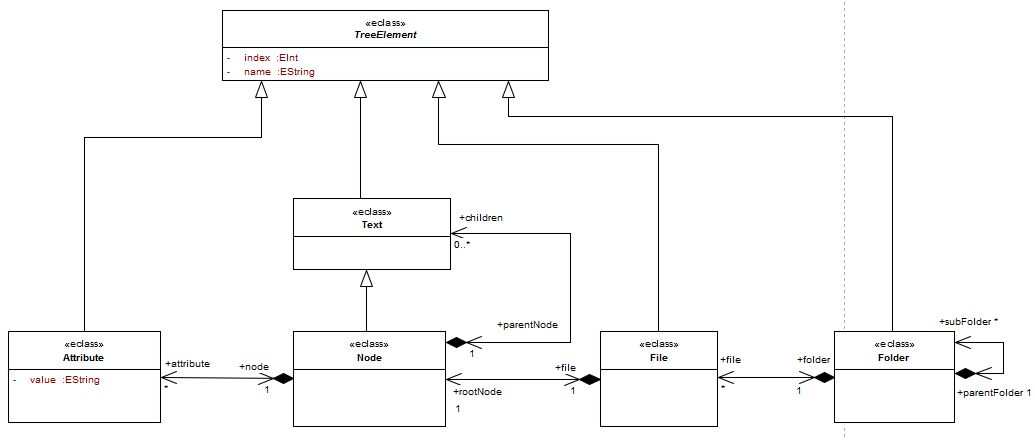
\includegraphics[width=\textwidth]{pics/moca/0Install/0-MocaTree}
  \caption{\texttt{Mocatree} Metamodel}
  \label{fig:moca-tree}
\end{center}
\end{figure}
 
\begin{enumerate}

\item[$\blacktriangleright$] Add a new package \texttt{DictionaryLanguage} and model the required classes and relationships for our dictionary language (Fig.~\ref{fig:moca-5-DictionaryMM}).

Every dictionary has a title and consists of entries.
Entries have a content and a level that indicates how difficult the entry is.
Dictionaries can be organized in shelves that have a description and shelves can be collected in a library.
To make things interesting, each dictionary has an author.
Note that arbitrary many different dictionaries, irrespective of their shelves, can share the same author.

%\usepackage{graphics} is needed for \includegraphics
\begin{figure}[!htbp]
\begin{center}
 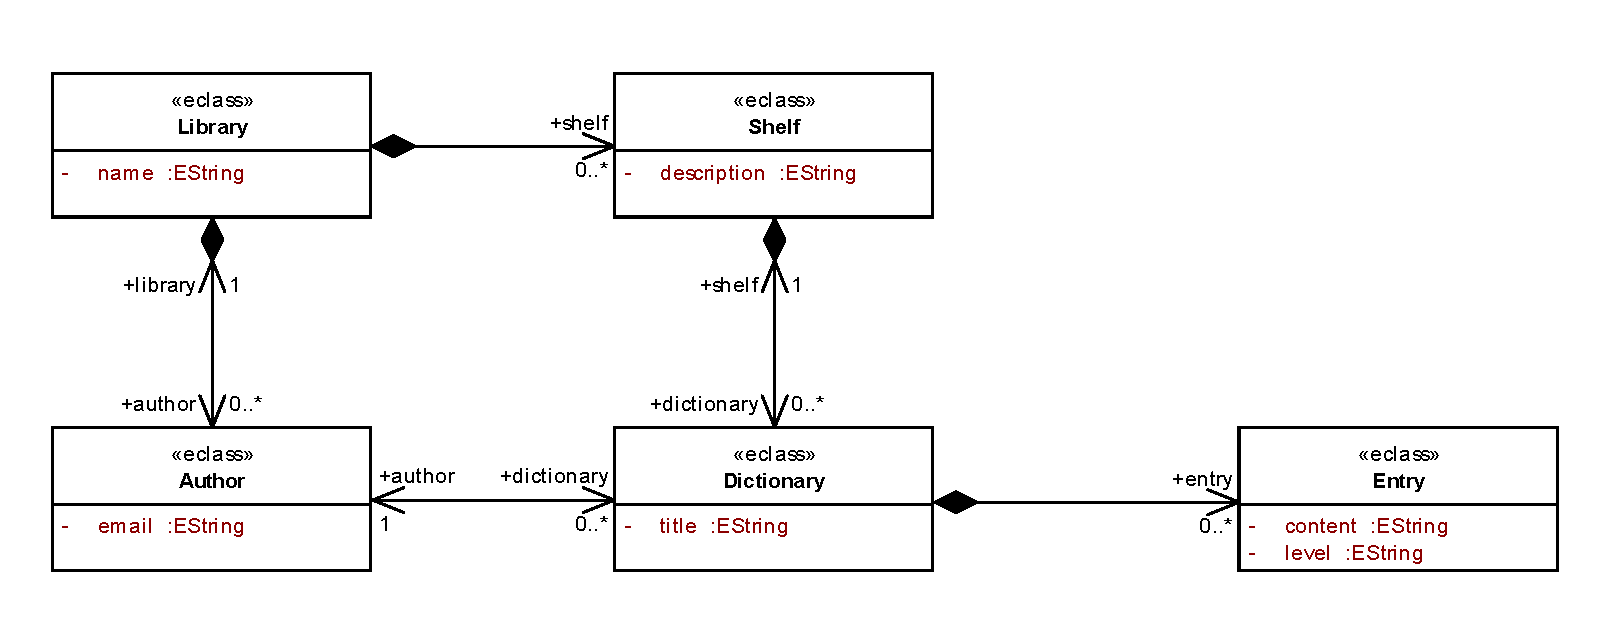
\includegraphics[width=0.9\textwidth]{pics/moca/1DictionaryMetaModel/DictionaryLanguage}
  \caption{Dictionary Metamodel}
  \label{fig:moca-5-DictionaryMM}
\end{center}
\end{figure}

\item[$\blacktriangleright$] For the moment, add an empty package in EA named \texttt{Dic\-tion\-ary\-Code\-Adapter} so that your EA workspace closely resembles Fig.~\ref{fig:moca-5-DictionaryMM-ProjectBrowser}.

According to our conventions and workflow, a \emph{code adapter} is a package that contains the tree-to-model transformation logic.
This could of course be integrated directly in the corresponding metamodel (\texttt{Dic\-tion\-ary\-Language} in our case), but a separation makes sense as there could be \emph{different} code adapters for the \emph{same} language.


%\usepackage{graphics} is needed for \includegraphics
\begin{figure}[!htbp]
\begin{center}
 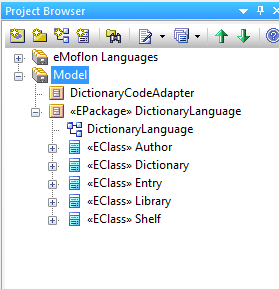
\includegraphics[width=0.25\textwidth]{pics/moca/1DictionaryMetaModel/5-DictionaryMM-ProjectBrowser.png}
  \caption{EA workspace before exporting}
  \label{fig:moca-5-DictionaryMM-ProjectBrowser}
\end{center}
\end{figure}

\item[$\blacktriangleright$] Export as usual and ensure that your Eclipse workspace closely resembles Fig.~\ref{fig:moca-6-ExportToEclipse}.
Note especially the library nodes (\texttt{Moflon} and \texttt{Moca}) that reference jars for all required dependencies. (If your \texttt{DictionaryCodeAdapter} is not exported or you receive an error message while exporting it, you can add an empty diagram to it)

%\usepackage{graphics} is needed for \includegraphics
\begin{figure}[!htbp]
\begin{center}
 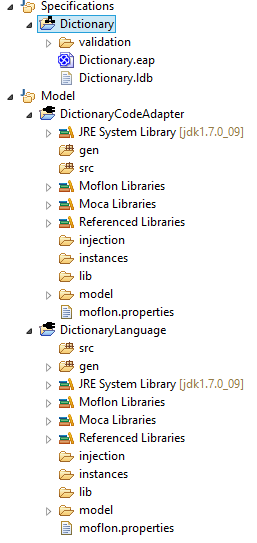
\includegraphics[width=0.25\textwidth]{pics/moca/1DictionaryMetaModel/6-ExportToEclipse.png}
  \caption{Workspace after export to Eclipse}
  \label{fig:moca-6-ExportToEclipse}
\end{center}
\end{figure}

\item[$\blacktriangleright$] Right-click on \texttt{DictionaryCodeAdapter} one more time and choose ``Add Parser/Unparser'', this time from the eMoflon context menu (Fig \ref{fig:moca-1-AddParserAndUnparserWizard}).

%\usepackage{graphics} is needed for \includegraphics
\begin{figure}[!htbp]
\begin{center}
 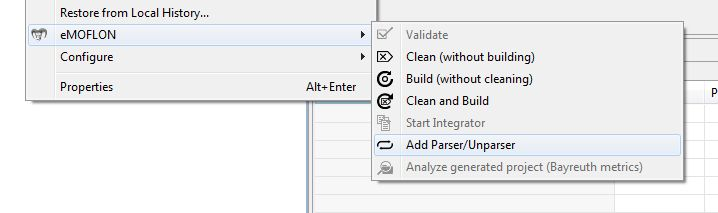
\includegraphics[width=0.75\textwidth]{pics/moca/2TextToMocaTree/1-AddParserAndUnparserWizard}
  \caption{Invoking the \texttt{Add Parser/Unparser} wizard} 
  \label{fig:moca-1-AddParserAndUnparserWizard}
\end{center}
\end{figure}
 
\item[$\blacktriangleright$] In the wizard dialogue (Fig \ref{fig:moca-2-AddParser}), enter ``dictionary'' as file extension, and check the boxes \texttt{Create Parser} and \texttt{Create Unparser} with \texttt{ANTLR} chosen as corresponding technology in both cases.  Click \texttt{Finish}. 

%\usepackage{graphics} is needed for \includegraphics
\begin{figure}[!htbp]
\begin{center}
 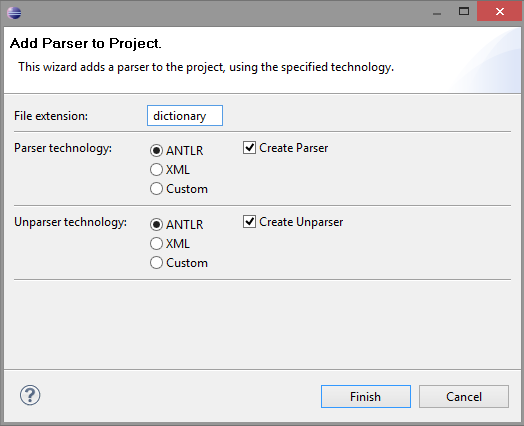
\includegraphics[width=0.6\textwidth]{pics/moca/2TextToMocaTree/2-AddParser.png}
  \caption{Add Parser/Unparser}
  \label{fig:moca-2-AddParser}
\end{center}
\end{figure}

\end{enumerate}

If everything has been installed and set up properly, parser and unparser stubs should be generated and \texttt{ANTLR} should automatically build the corresponding Java code as depicted in Fig.~\ref{fig:moca-3-WizardResult}. 

%\usepackage{graphics} is needed for \includegraphics
\begin{figure}[!htbp]
\begin{center}
 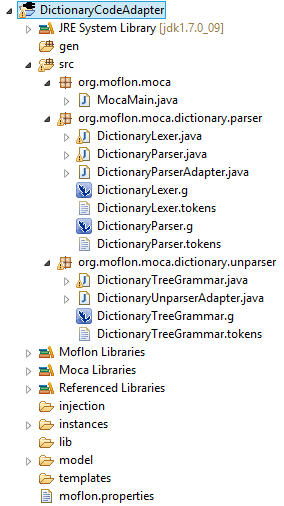
\includegraphics[width=0.65\textwidth]{pics/moca/2TextToMocaTree/3-WizardResult.png}
  \caption{Workspace after wizard finishes}
  \label{fig:moca-3-WizardResult}
\end{center}
\end{figure}
